\documentclass[portrait,final,a0paper,fontscale=0.3]{baposter}

\usepackage[utf8]{inputenc}
\usepackage[T1]{fontenc}
\usepackage[frenchb]{babel} 

\usepackage{graphicx}
\usepackage{multirow}
\usepackage{enumitem}
\usepackage{url}

\usepackage{graphicx}
\usepackage{multicol}

\usepackage{palatino}

\usepackage{wasysym}

\newcommand{\captionfont}{\footnotesize}

\frenchbsetup{ItemLabeli=\textbullet}
\frenchbsetup{ItemLabelii=\normalfont \bfseries \textendash}
\frenchbsetup{ItemLabeliii=\textasteriskcentered}
\frenchbsetup{ItemLabeliv=\textperiodcentered}

% Multicol Settings
%%%%%%%%%%%%%%%%%%%%%%%%%%%%%%%%%%%%%%%%%%%%%%%%%%%%%%%%%%%%%%%%%%%%%%%%%%%%%%%%
\setlength{\columnsep}{1.5em}
\setlength{\columnseprule}{0mm}

%%%%%%%%%%%%%%%%%%%%%%%%%%%%%%%%%%%%%%%%%%%%%%%%%%%%%%%%%%%%%%%%%%%%%%%%%%%%%%%%
\newcommand{\compresslist}{%
\setlength{\itemsep}{1pt}%
\setlength{\parskip}{0pt}%
\setlength{\parsep}{0pt}%
}
\setlist{leftmargin=5.5mm}

\definecolor{darkblue}{rgb}{0.1,0.2,0.5}
\definecolor{darkred}{rgb}{0.7,0,0.0}
\definecolor{darkgreen}{rgb}{0.0,0.4,0.0}
\definecolor{darkmagenta}{rgb}{0.4,0.0,0.4}
\definecolor{darkcyan}{rgb}{0.0,0.5,0.5}
\definecolor{darkyellow}{rgb}{1,0.5,0.0}
\definecolor{darkgray}{rgb}{0.2,0.2,0.2}
\definecolor{lightgray}{rgb}{0.9,0.9,0.9}
\definecolor{verylightgray}{rgb}{0.95,0.95,0.95}
\definecolor{ensggreen}{rgb}{0.50,0.63,0.05}
\definecolor{ensggray}{rgb}{0.45,0.47,0.49}
\definecolor{lightgreen}{rgb}{0.0,0.9,0.0}
\definecolor{lightred}{rgb}{0.9,0.0,0.0}
\definecolor{lightblue}{rgb}{0.0,0.0,0.9}


\renewenvironment{emph}[1]{\textbf{#1}}{}

\begin{document}

\hyphenation{resolution occlusions}
\begin{poster}%
	% Poster Options
	{
	columns=6,
	% Column spacing
	colspacing=0.7em,
	% Color style
	bgColorOne=white,
	borderColor=darkblue,
	headerColorOne=darkblue,
	headerFontColor=white,
	boxColorOne=white,
	% Format of textbox
	textborder=roundedsmall,
	% Format of text header
	headerborder=closed,
	headerheight=0.1\textheight,
	%  textfont=\sc, An example of changing the text font
	headershape=smallrounded,
	headershade=plain, %shadelr,
	headerfont=\Large\bf\textsc, %Sans Serif
	textfont={\setlength{\parindent}{1.5em}},
	boxshade=plain,
	background=plain, %shadetb
	linewidth=2pt
	}
	% Logo1
	{
\includegraphics[height=9.0em]{ensta_bzh.png}} 
	% Title
	{\bf\textsc{Évaluation d'une solution de positionnement ponctuel précis temps-réel}\vspace{0.5em}}
	% Authors
	{\normalsize\textsc{Pierre BOSSER$^{(1,2)}$, Ismail HMAMA$^{(1)}$ Iiro KUUSISTO$^{(1)}$, Julien Le MERCIER$^{(1)}$, Christelle MEKEM LANDO$^{(1)}$}\vspace{0.5em}
	\\(1) ENSTA Bretagne, Brest, France ; (2) Lab-STICC, Brest, France
	\vspace{-0.25cm}}
	% Logo2
	{}

%%%%%%%%%%%%%%%%%%%%%%%%%%%%%%%%%%%%%%%%%%%%%%%%%%%%%%%%%%%%%%%%%%%%%%%%%%%%%%
\headerbox{Contexte}{name=contexte,column=0,span=4}{
%%%%%%%%%%%%%%%%%%%%%%%%%%%%%%%%%%%%%%%%%%%%%%%%%%%%%%%%%%%%%%%%%%%%%%%%%%%%%%
	\setlength{\parindent}{0pt}
	Le positionnement différentiel en temps réel (RTK) est la technique de positionnement GNSS en temps réel la plus utilisée actuellement. De précision centimétrique, elle s'est largement développée en particulier avec la mise en place des réseaux RTK (N-RTK). 
	
	\smallskip
	La principale faiblesse de ce mode de positionnement par GNSS est la nécessité de disposer d'une ou plusieurs stations de référence, de préférence proche, pour une précision optimale. D'un autre coté, le positionnement ponctuel précis par GPS (PPP), apparu dans les milieux scientifiques dans les années 1990, s'est largement développé au cours des années 2000. Il présente l'avantage de fournir une position en mode absolu, c'est-à-dire calculée indépendamment de toute station de référence.
}

\headerbox{Objectifs}{name=resume,column=4,span=2}{
	\setlength{\parindent}{0pt}
	
	\vspace{2mm}
	\begin{center}
		\textcolor{red}{\emph{Évaluation du PPP temps réel RTX de Trimble
		\\(\textit{Real Time eXtended})}}
	\end{center}
	
	\vspace{-1mm}
	Critères testés :
	\begin{itemize}
		\item Initialisation de la solution.
		\item Performances en positionnement statique.
		\item Performances en positionnement dynamique.
	\end{itemize}
}

\headerbox{Méthodologie}{name=methodologie,column=0,below=contexte,span=6}{
	\setlength{\parindent}{0pt}
	\centering Quatre type de positionnement GPS sont considérés (2 en temps réel, 2 en temps différé ; 2 absolus, 2 différentiels).
	
	\begin{minipage}[t]{0.24\textwidth}
		\vspace{-0.1cm}
		\begin{center}
			\large\textcolor{red}{\emph{R T X}}
		\end{center}
		\small\vspace{-0.4cm}
		\begin{itemize}
			\item Récepteur SPS855.
			\item Antenne Antcom.
			\item Calcul temps réel RTX Trimble.
			\item Positions à 1~s ou 30~s.
			\item Positions exprimées en ITRF08 puis ramenées en RGF93.
		\end{itemize}
	\end{minipage}
	\begin{minipage}[t]{0.24\textwidth}
		\vspace{-0.1cm}
		\begin{center}
			\large\textcolor{blue}{\emph{P P P}}
		\end{center}
		\small\vspace{-0.4cm}
		\begin{itemize}
			\item Récepteur SPS855.
			\item Antenne Antcom.
			\item Post-traitement : calcul PPP sous Gipsy-Oasis 6.4 (IERS 2013, ambiguïtés entières).
			\item Positions à 1~s ou 30~s.
			\item Positions exprimées en ITRF08 puis ramenées en RGF93.
		\end{itemize}
	\end{minipage}
	\begin{minipage}[t]{0.24\textwidth}
		\vspace{-0.1cm}
		\begin{center}
			\large\textcolor{green}{\emph{R T K}}
		\end{center}
		\small\vspace{-0.4cm}
		\begin{itemize}
			\item Proflex 500.
			\item Antenne Magellan MAG111406.
			\item Calcul temps réel N-RTK (Teria).
			\item Positions à 1~s ou 30~s.
			\item Positions exprimées en RGF93, ramenées au niveau de l'antenne RTX Trimbe en post-traitement.
		\end{itemize}
	\end{minipage}
	\begin{minipage}[t]{0.24\textwidth}
		\vspace{-0.1cm}
		\begin{center}
			\large\textcolor{cyan}{\emph{D D}}
		\end{center}
		\small\vspace{-0.4cm}
		\begin{itemize}
			\item Récepteur SPS855.
			\item Antenne Antcom.
			\item Post-traitement : calcul différentiel sous RTKlib 1.4.3.
			\item Positions à 1~s ou 30~s.
			\item Positions exprimées en RGF93 à partir des stations BRST et GUIP (RGP).
		\end{itemize}
	\end{minipage}
}

\headerbox{Initialisation}{name=initialisation,column=0,below=methodologie,span=3}{
	\setlength{\parindent}{0pt}
	\begin{itemize}
		\item 6 sessions d'1 h pour différentes configurations de satellites.
		\item Utilisation du \textcolor{red}{RTX} seul.
	\end{itemize}

	\vspace{-2mm}
	\centering
	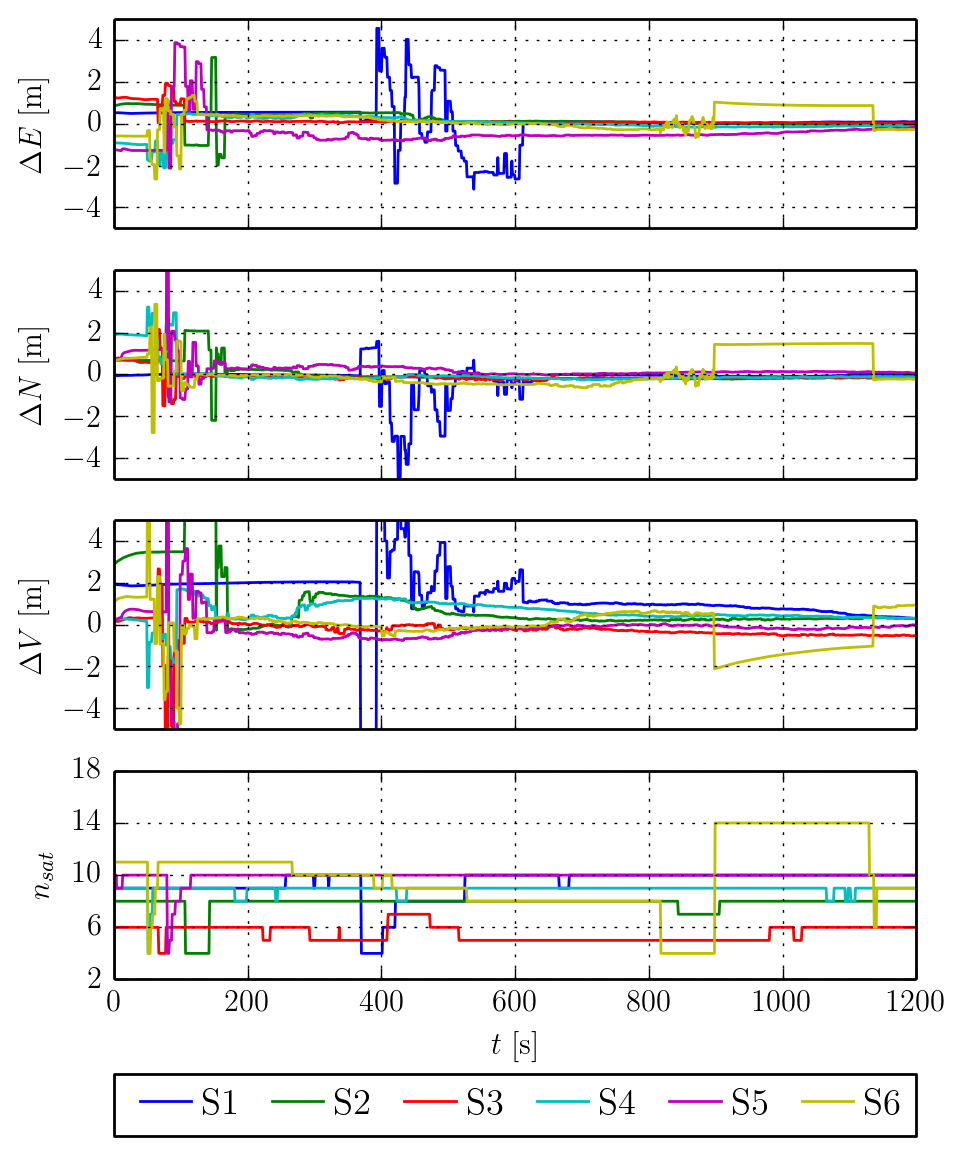
\includegraphics[width=5.5cm]{figures/1_init_large.png}
	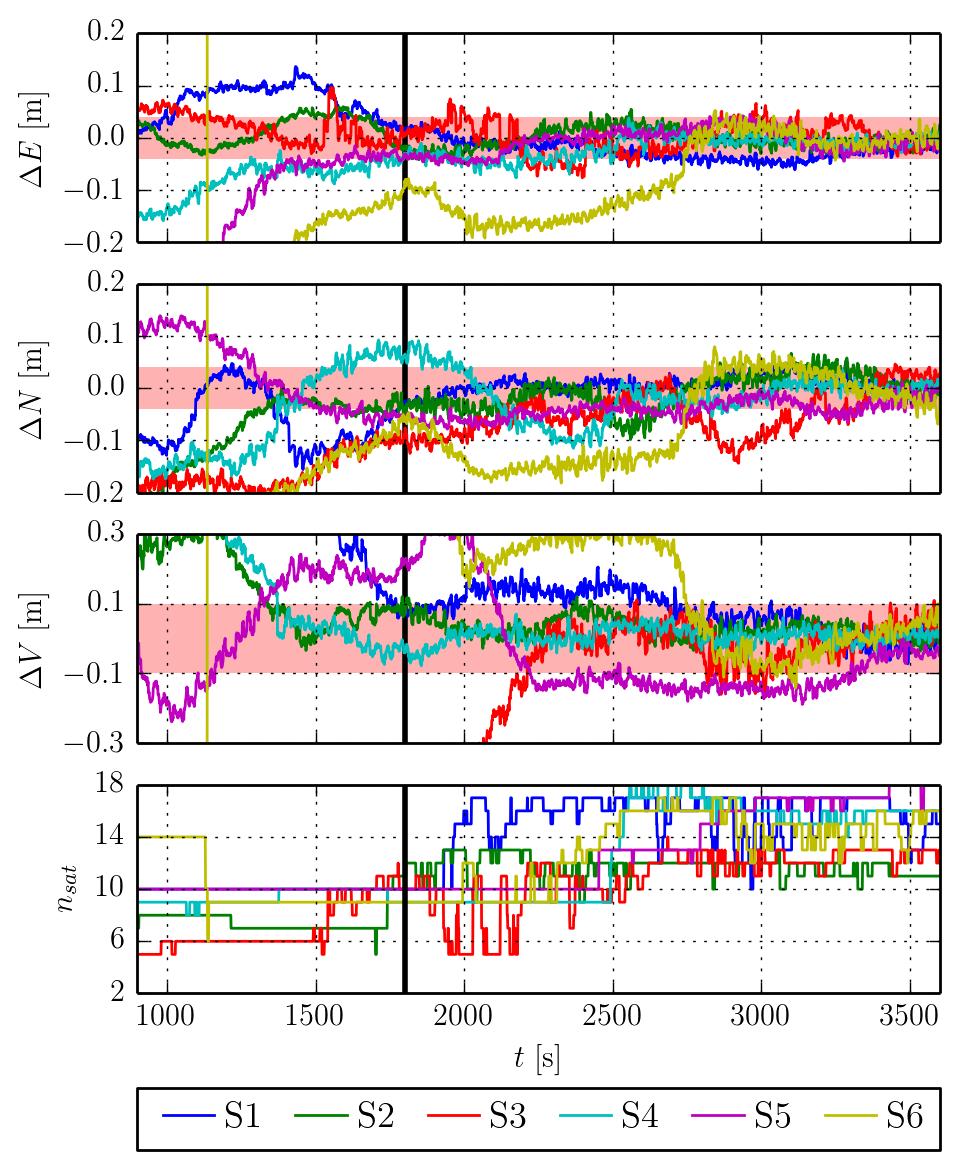
\includegraphics[width=5.5cm]{figures/2_init_tight.png}
	
	\vspace{-1mm}
	{\footnotesize\it Convergence des solutions pour les 4 méthodes (début et fin de session).}

	\vspace{-2mm}
	\begin{center}
	\begin{tabular}{cccccrrr}
		\hline
		S & Date  & Début & Fin   & $N_{sat}$ & $\sigma_E$ [cm] & $\sigma_N$ [cm] & $\sigma_U$ [cm]\\
		\hline
		1 & 24/11 & 12:40 & 13:40 & 4/17      & 1,7             & 1,5             &  6,0            \\
		2 & 24/11 & 13:42 & 14:42 & 4/13      & 1,8             & 3,3             &  2,8            \\
		3 & 24/11 & 14:40 & 15:45 & 4/14      & 2,9             & 4,3             & 15,3            \\
		4 & 27/11 & 07:26 & 08:26 & 4/18      & 2,0             & 4,1             &  2,5            \\
		5 & 02/12 & 09:00 & 10:00 & 4/18      & 2,3             & 1,8             & 14,1            \\
		6 & 02/12 & 10:04 & 11:04 & 4/17      & 7,4             & 7,9             & 18,7            \\
		\hline
	\end{tabular}
	
	\vspace{2mm}
	{\footnotesize\it Répétitivités après initialisation théorique (30 min.).}
	\end{center}
}

\headerbox{Positionnement statique}{name=statique,column=0,below=initialisation,span=3}{
	\setlength{\parindent}{0pt}
	\begin{minipage}[c]{0.5\textwidth}
		\begin{itemize}
			\item Positions à 30~s calculées pendant 3 jours.
			\item Positions de référence issues du traitement \textcolor{cyan}{DD}.
		\end{itemize}
		
		\centering
		\begin{tabular}{crrr}
			\hline
			 & $\sigma_E$ [cm] & $\sigma_N$ [cm] & $\sigma_U$ [cm]\\
			\hline
			\textcolor{red}{RTX}   & 3,2 & 2,2 & 6,8 \\
			\textcolor{blue}{PPP}  & 1,3 & 1,6 & 2,1 \\
			\textcolor{green}{RTK} & 1,3 & 1,8 & 4,2 \\
			\textcolor{cyan}{DD}   & 0,8 & 1,2 & 1,4 \\
			\hline
		\end{tabular}
		
		\smallskip
		{\footnotesize\it Répétitivité sur la période.}\\
		
		\medskip
		\small
		\begin{tabular}{crrr}
			\hline
			 & $\Delta E$ [cm] & $\Delta N$ [cm]& $\Delta U$ [cm]\\
			\hline
			\textcolor{red}{RTX}   &  1,5 $\pm$ 3,3 &  0,1 $\pm$ 2,3 & 7,4 $\pm$ 7,7\\
			\textcolor{blue}{PPP}  &  0,0 $\pm$ 1,6 & -1,8 $\pm$ 1,9 & 0,0 $\pm$ 3,5\\
			\textcolor{green}{RTK} & -0,1 $\pm$ 1,4 &  0,7 $\pm$ 1,9 & 1,0 $\pm$ 4,4\\
			\hline
		\end{tabular}
		
		\smallskip
		{\footnotesize\it Écarts par rapport au calcul \textcolor{cyan}{DD}}.\\
	\end{minipage}
	\begin{minipage}[c]{0.49\textwidth}
		\centering
		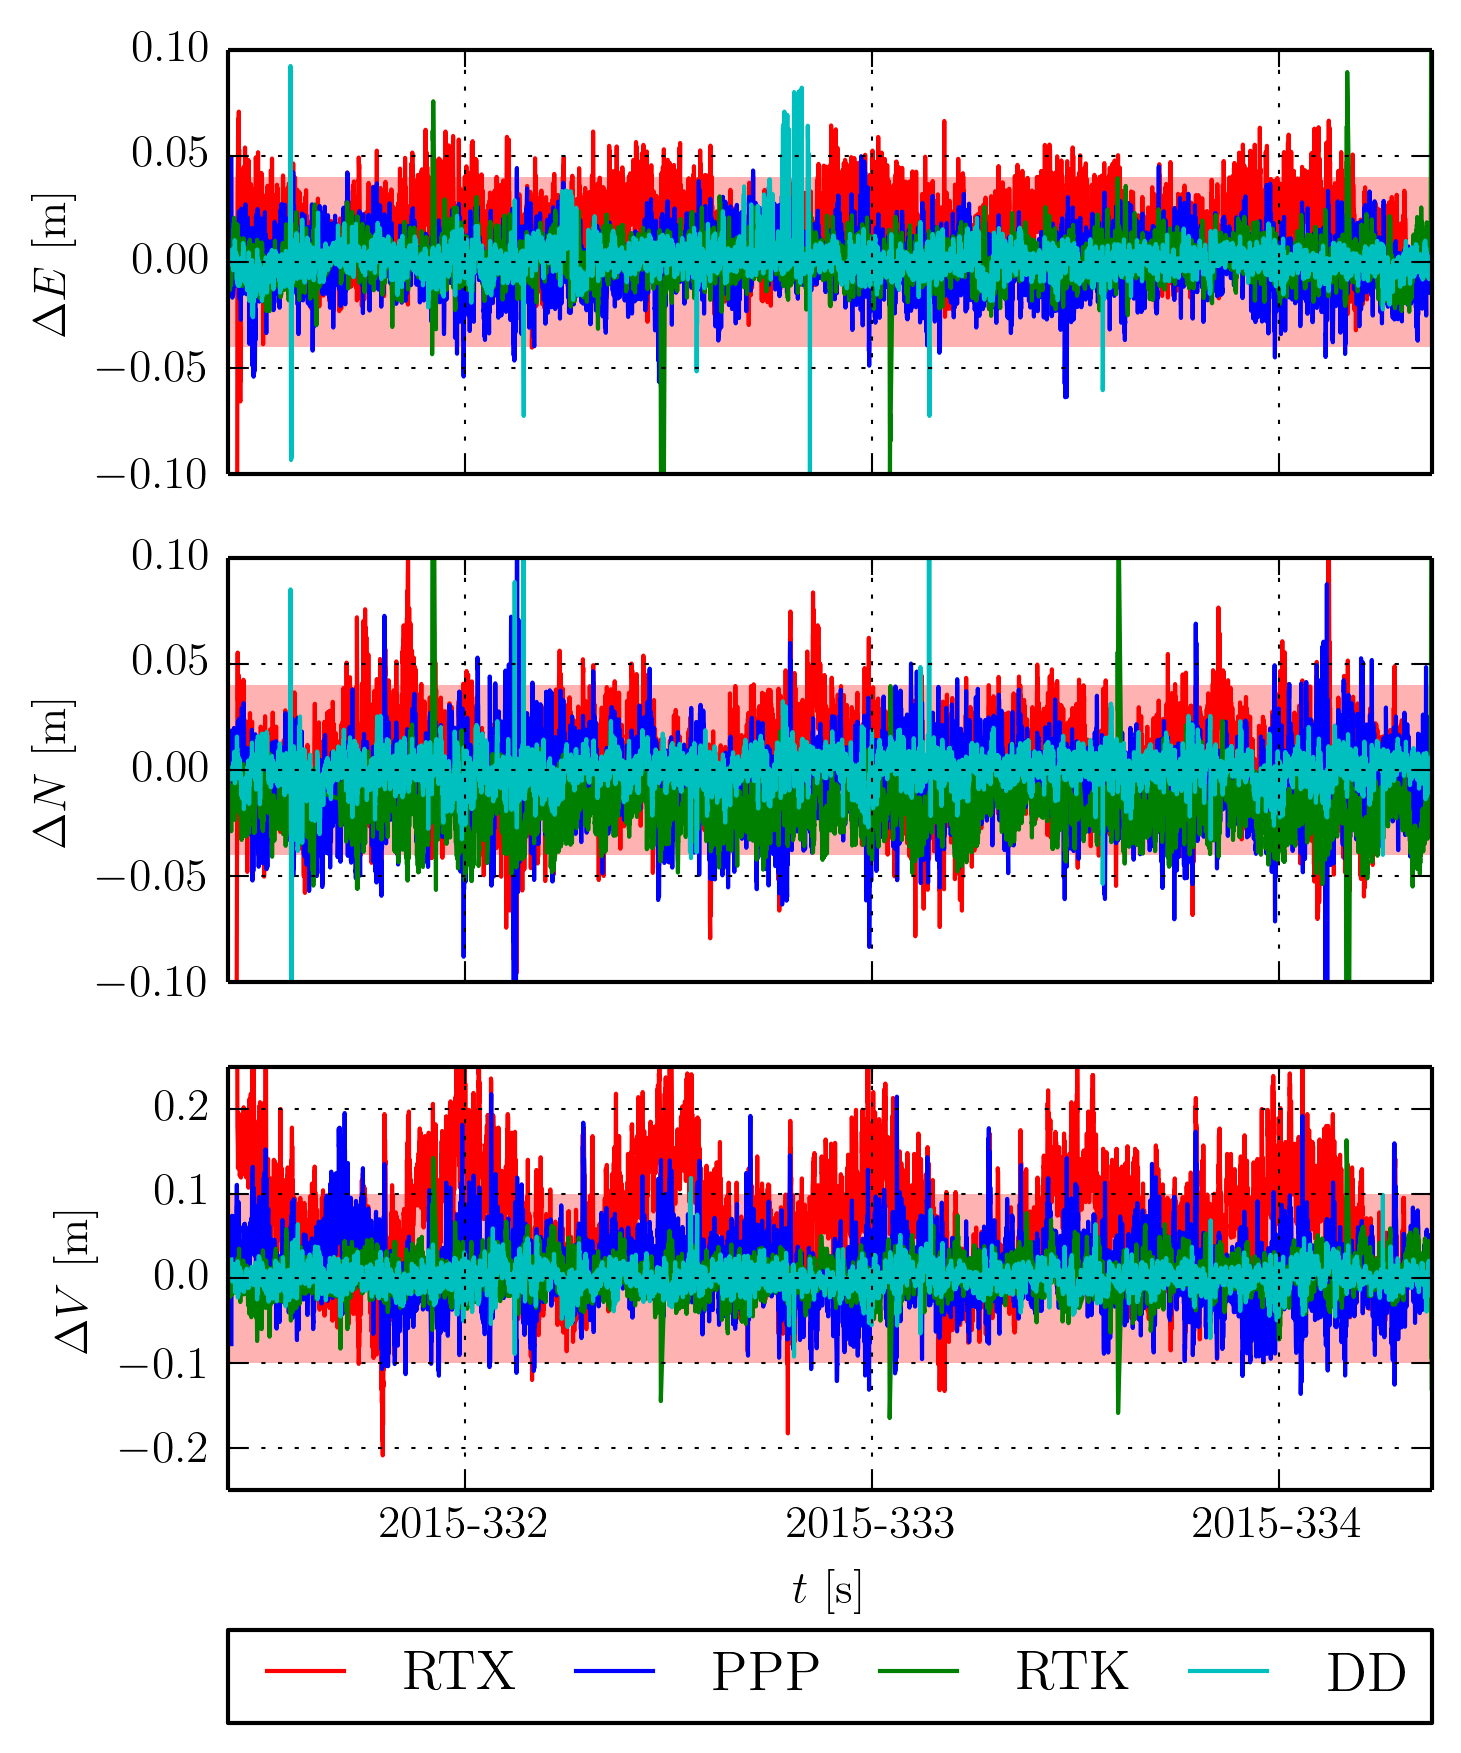
\includegraphics[width=5.5cm]{figures/3_statique.png}
		
		\vspace{-0.2cm}
		{\footnotesize\it Écarts à la position de référence.}\\
	\end{minipage}

}

\headerbox{Positionnement dynamique}{name=dynamique,column=3,below=methodologie,span=3}{
	\setlength{\parindent}{0pt}
	
	\begin{minipage}{0.55\textwidth}
		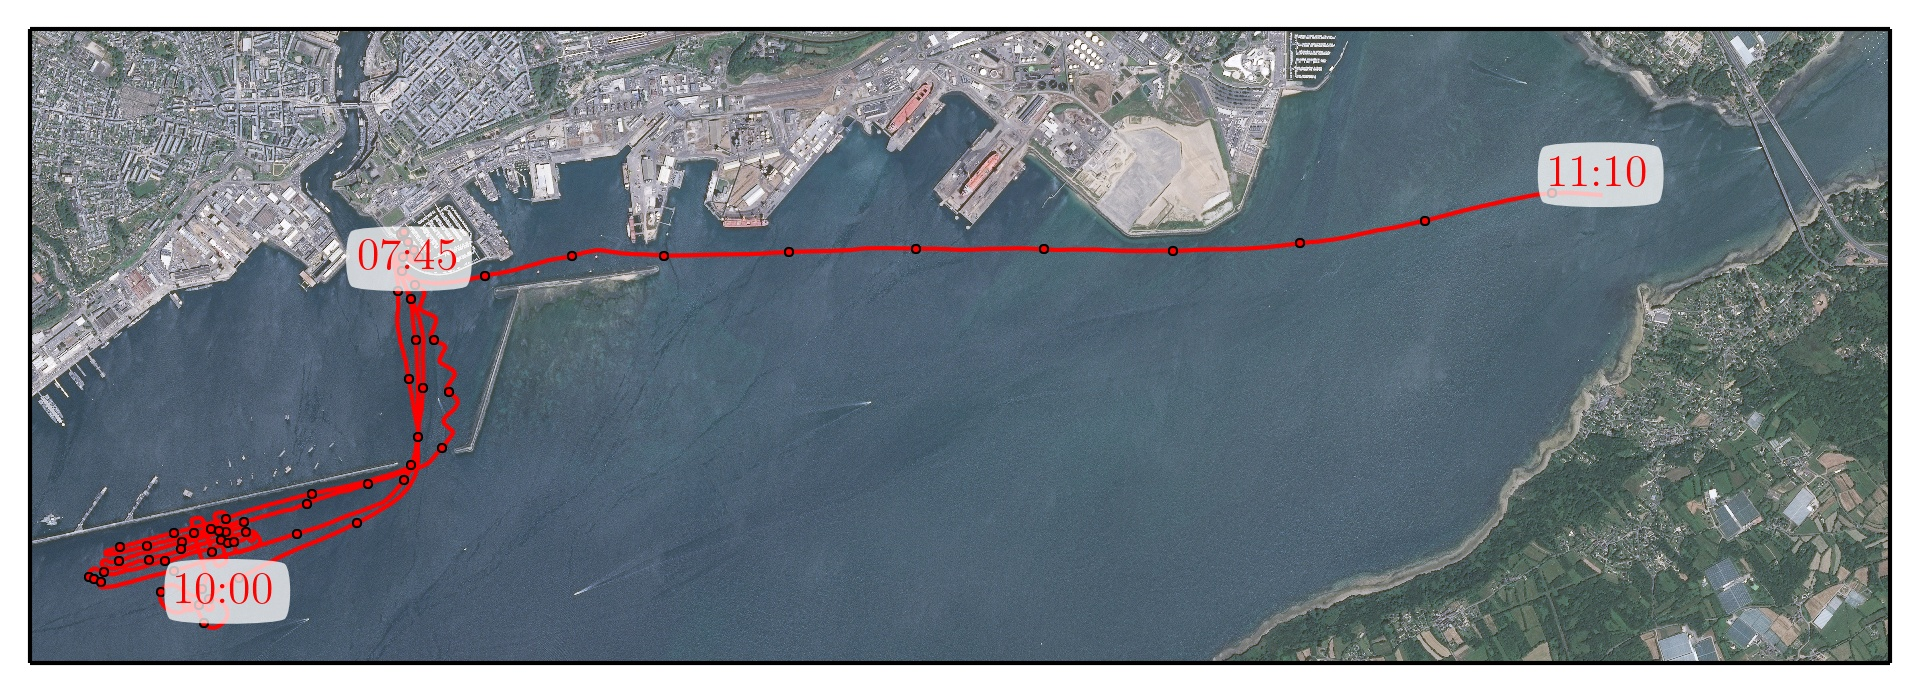
\includegraphics[width=6.5cm]{figures/4_map_survey.jpg}
	\end{minipage}
	\begin{minipage}{0.44\textwidth}
		\begin{itemize}
			\item Levé hydrographique en rade de Brest (environnement dégagé et faible vitesse).
			\item Positions à 1~s.
			\item Positions de référence issues du traitement \textcolor{cyan}{DD}.
		\end{itemize}
	\end{minipage}
	
	\medskip
	\begin{minipage}[c]{0.52\textwidth}
		\centering
		\small
		\begin{tabular}{crrr}
			\hline
			 & $\Delta E$ [cm] & $\Delta N$ [cm]& $\Delta U$ [cm]\\
			\hline
			\textcolor{red}{RTX}   &  3,2 $\pm$ 5,7 & -0,3 $\pm$ 7,5 & 10,7 $\pm$ 17,8\\
			\textcolor{blue}{PPP}  &  0,3 $\pm$ 0,8 &  1,0 $\pm$ 1,0 &  1,7 $\pm$  1,9\\
			\textcolor{green}{RTK} &  0,2 $\pm$ 0,9 & -0,2 $\pm$ 1,1 & -6,2 $\pm$ 2,3\\
			\hline
		\end{tabular}
		
		\begin{center}
			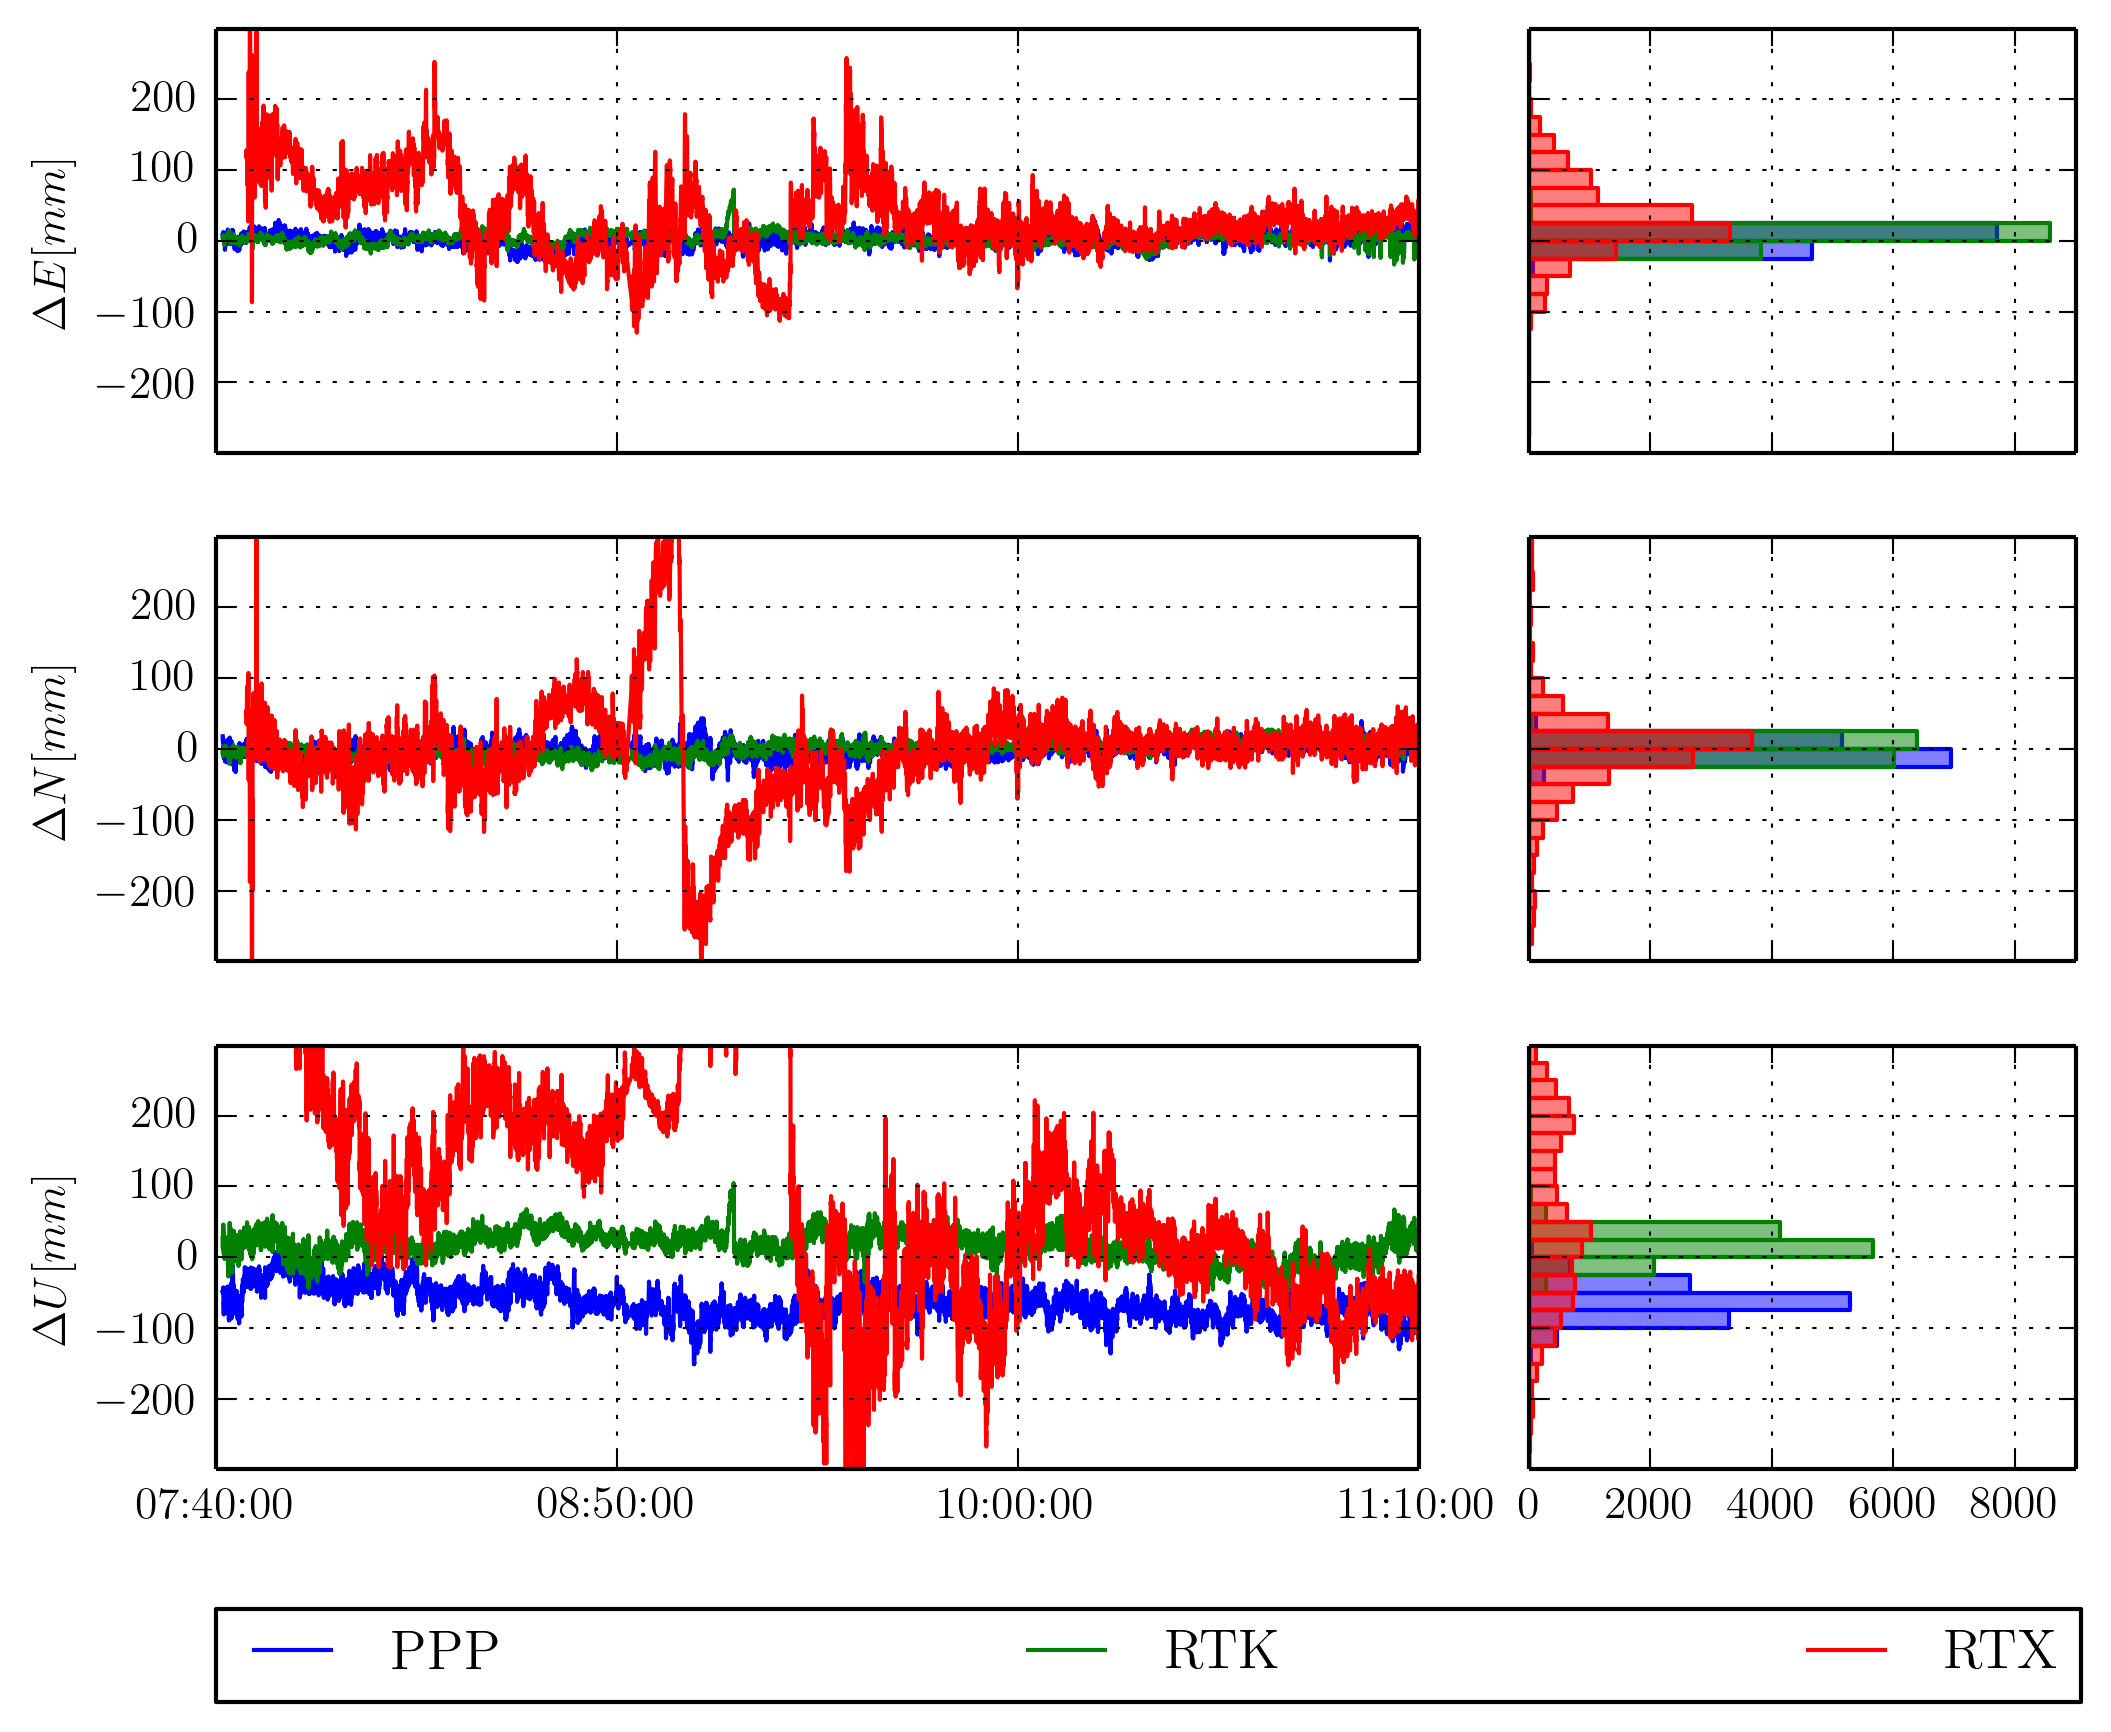
\includegraphics[width=5.5cm]{figures/5_survey_cmp.png}
			{\footnotesize\it Écarts par rapport au calcul \textcolor{cyan}{DD}.}
		\end{center}
	\end{minipage}
	\hspace{1.1mm}
	\begin{minipage}[c]{0.47\textwidth}
		\vspace{5mm}\centering
		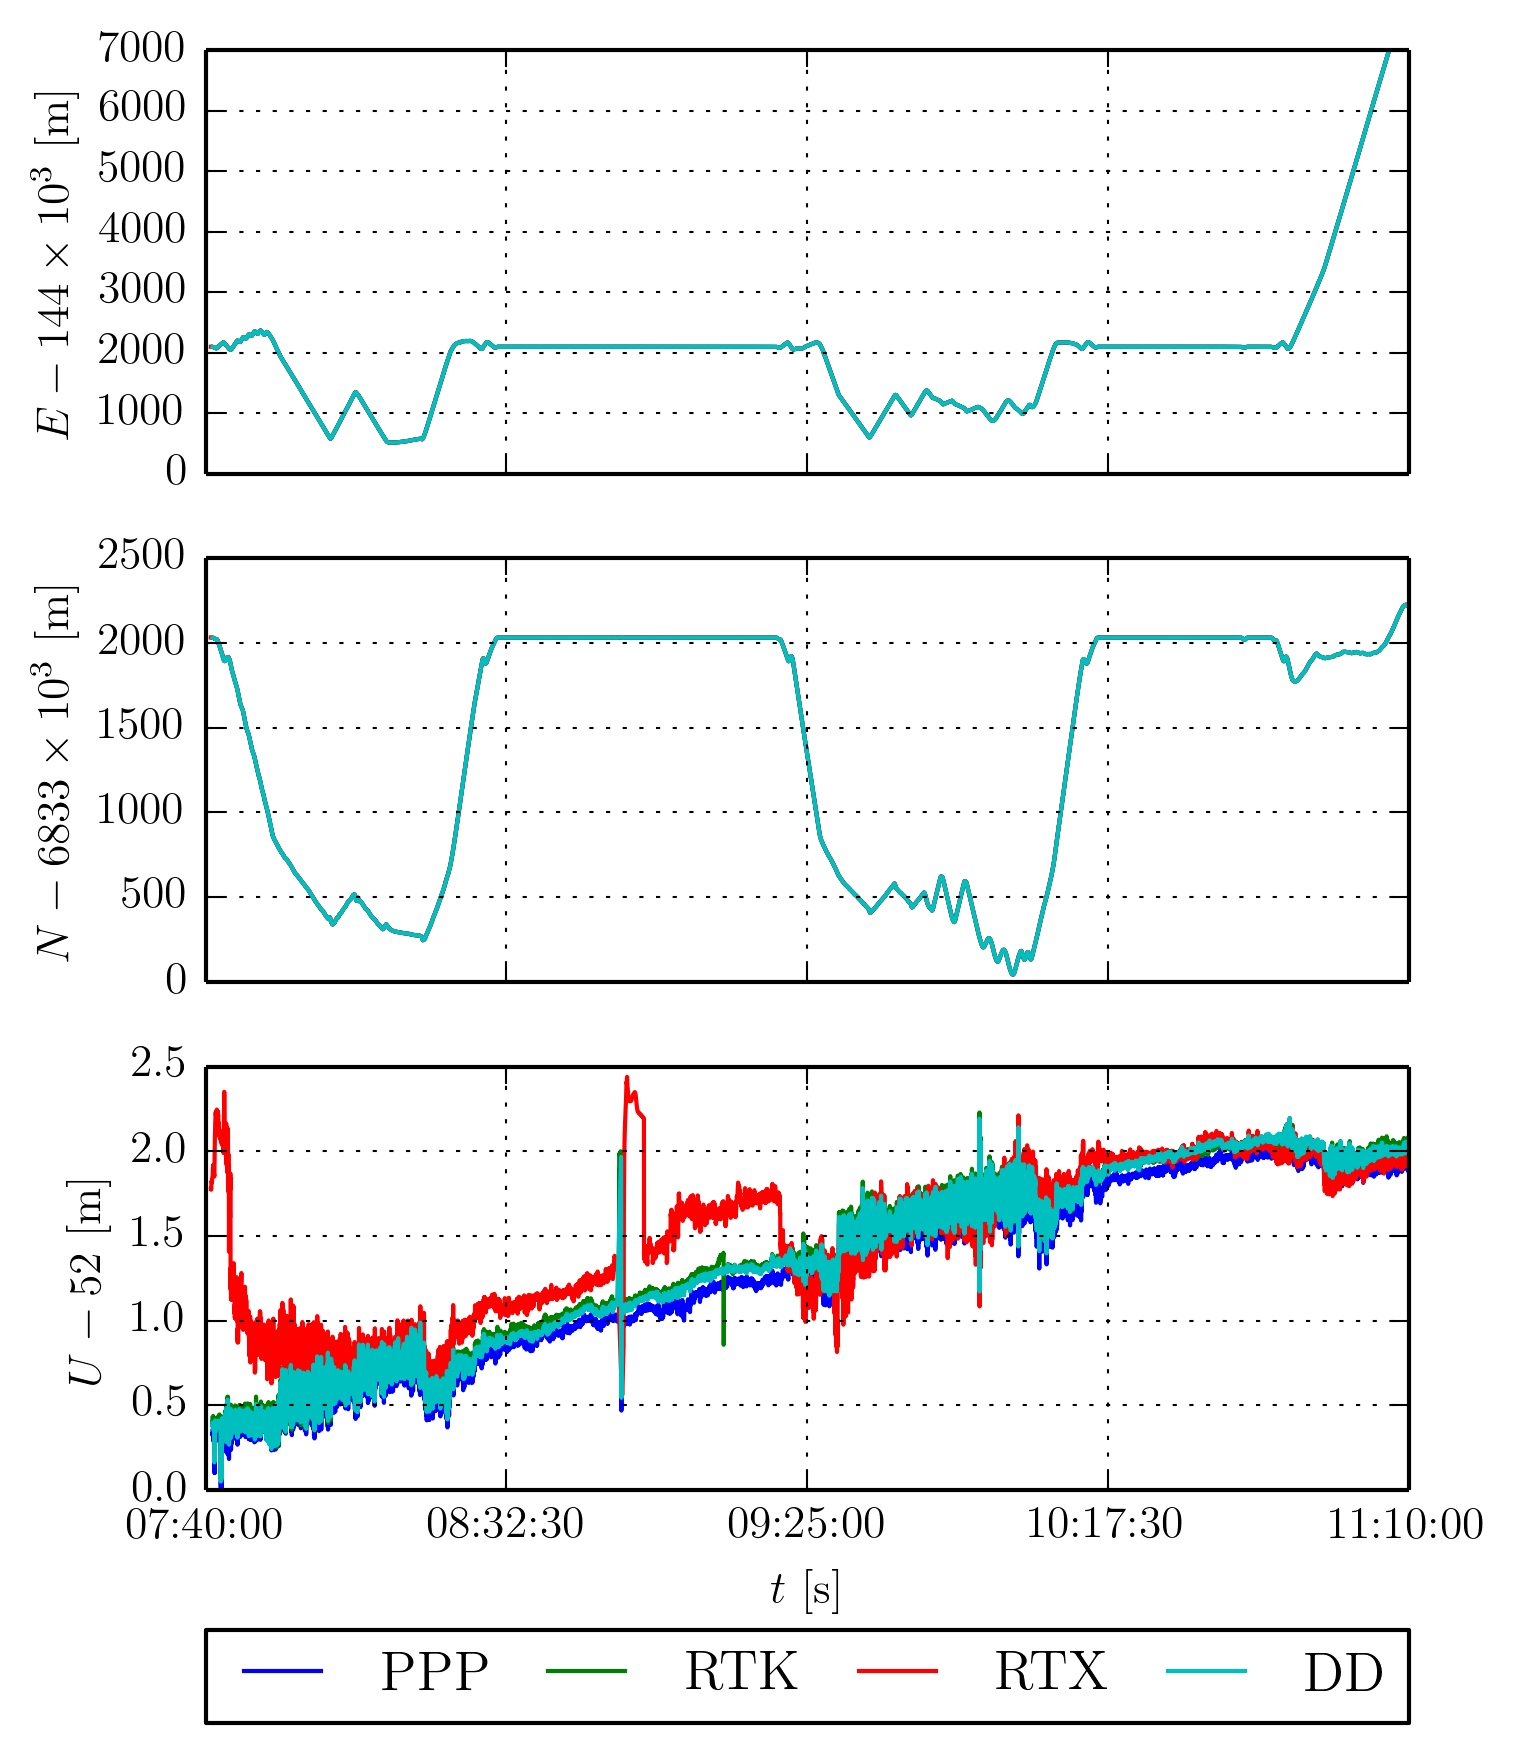
\includegraphics[width=5.5cm]{figures/6_survey_hydro.png}
		\footnotesize\it Positions instantanées par méthode.
	\end{minipage}
}

\headerbox{Conclusion}{name=conclusion,column=3,below=dynamique, span=3}{
	\setlength{\parindent}{0pt}
	\smallskip
	\centering\emph{Confirmation des spécifications annoncées}.
	\smallskip
	\begin{description}[nolistsep]
		\item\textcolor{green}{\smiley} Durée de convergence confirmée, environ 30 min.
		\item\textcolor{green}{\smiley} Précisions confirmées (4 cm en horizontal, 10 cm en vertical).
		\item\textcolor{green}{\smiley} Mise en application simple.
		\smallskip
		\item\textcolor{red}{\frownie} Convergence parfois allongée.
		\item\textcolor{red}{\frownie} Perte ponctuelle d'initialisation.
		\item\textcolor{red}{\frownie} Variations périodiques sur la verticale.
		\item\textcolor{red}{\frownie} Dégradation des précisions en levé dynamique.
	\end{description}
	\smallskip
}

\headerbox{}{name=conclusion,column=3,below=conclusion, span=3}{
	\setlength{\parindent}{0pt}\small\smallskip
	Les auteurs tiennent à remercier :
	\begin{itemize}
		\item La société PrimeGPS pour la mise à disposition du système RTX.
		\item Le réseau Teria pour la mise à disposition d'un abonnement N-RTK.
		\item Pierre Simon (ENSTA Bretagne) pour son soutien technique et logistique.
	\end{itemize}
	
	\vspace{0.03cm}
	Cette étude a été réalisée durant l'année scolaire 2015-2016 dans le cadre du projet de 3ème année du cycle Ingénieur de l'ENSTA Bretagne, spécialité "Hydrographie et Océanographie".
}

\end{poster}
\end{document}